\chapter*{Introduction}
\addcontentsline{toc}{chapter}{Introduction}

Imagine, for a moment, that you are transported in time to 10th-century Europe. It is Sunday, and the weekly mass is just
starting. Look around yourself. The tall ceilings of the impressive church were built so to bring you closer to God. The stained glass windows
let through just enough light so that it is not completely dark. Can you smell the incense? Everything in the environment around
you reminds you that you are taking part in a sacred ritual. Listen to the priest; when he recites the prayers, his speech does not 
flow in a natural way. Instead, the entire text is intoned on a single note, except for the slightly inflected ends of clauses. 
Sometimes, the choir replaces the priest, singing more elaborate monophonic melodies. The words they are singing are Latin, but even 
if you do not understand them, you know what their purpose is: to celebrate the deity. Their voices echo in the stone church, creating an
otherwordly experience.

What you are hearing is called Gregorian chant. It is one of the earliest forms of music preserved in written form, and the
largest preserved body of medieval music. The earliest preserved fragments of written notes date back to the 9th century, although texts from as early as 
the eighth century have been found.. Its name, Gregorian, references Pope Gregory the Great, however, his relation to the chant is not entirely clear.

Gregorian chant is not the only type of chant. In the early centuries after Christianity spread across Western and Eastern Roman Empire,
new forms of worship started being developed. The most obvious differences were between the West and the East, which had multiple cultural
centers such as Constantinople, Jerusalem, or Alexandria. However, liturgies varied in the West as well, from Rome to Milan to the Iberian peninsula to Gaul.
Each center developed their own tradition, including their own type of chant. 

(TODO: why is the Roman tradition everywhere now?)

Gregorian chant is an integral part of the Roman church, and has been so for centuries. It is the monophonic music (i.e. single-voice)
sung during liturgies. Here, liturgy means chant sung during Christian worship. Unlike in the Eastern churches, where the term is reserved 
for the Eucharist, liturgy includes both the Mass and the Divine Office in the Roman church.

Mass is the service most familiar to most believers.
It can be divided into several parts, all leading up to the most important one, the act of communion. This act commemorates the Last Supper,
Jesus's last meal with his disciples before his execution. During the communion, bread, representing Christ's body, and wine, representing his
blood, are given out. During the course of the Mass, multiple different chants are sung. \emph{Introitus}, meaning 'entrance', is sung at the beginning
of the service while the priest and his assistants are walking to the altar. \emph{Tractus} is a chant that is sung during Lent, i.e. the period
between Ash Wednesday and the Saturday before Easter. Outside of this period, \emph{alleluia} replaces \emph{tractus} and is followed by \emph{sequentia}
on the most important feast days.

The other part of the liturgy, besides the Mass, is the Divine Office, also called Liturgy of the Hours or canonical hours. It is the set of chants
sung during services at different times of the day, for example \emph{Vespers} in the evening or \emph{Lauds} in the morning. The office consists
largely of singing psalms, of which there are 150, all sung on different days and hours. Psalms were usually preceded and followed by antiphons,
which differ not only by the day of the week, but also depending on the place. Each day of the week had an allocated set of antiphons, hymns and
responsories, while responsories were assigned to the different Sundays. Additionally, important feasts had their own set of chants to be sung.

The liturgical year contains several feasts. Some feasts are fixed on a specific date. Feasts associated with a specific saint are an example of those.
For example, John the Baptist is celebrated on the 24th of June, Michael on the 29th of September, and All Saints on the 1st of November. Other
fixed-date feasts include Christmas Day (25 December), Epiphany (6 January), and others. Such feasts can fall on any day of the week, and if they fall
on a Sunday, they will take precedence over it. On the other hand, there are also feasts that are fixed to a specific day of the week, the most important
of them being Easter Sunday, the day when Christ rose from the dead. Each feast has a different set of chants that can be completely original.

The individual chants differ in several criteria, the first one being the mode. Mode is the system of pitch organization, somewhat similar to modern-day
scales. Melodies are classified into one of eight modes according to their last note, called \emph{finalis}, and their range. Most chants
end on one of the notes \emph{D}, \emph{E}, \emph{F}, or \emph{G}. These four notes determine four pairs of modes. The melodies were further classified
depending on whether they moved mostly in the range above the \emph{finalis}, in which case it would be classified as the \emph{authentic} mode
of the pair, or in the range around the \emph{finalis}, which means it is classified as the \emph{plagal} mode. Some types of chant tend to
occur mostly in a specific mode.

\begin{figure}[h]
\centering
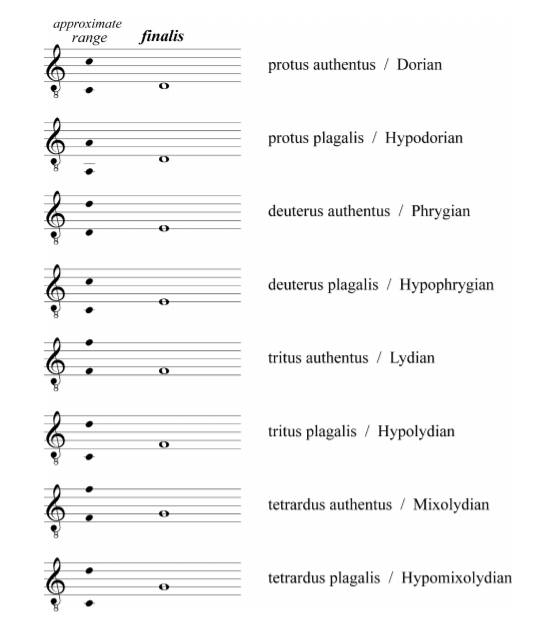
\includegraphics[scale=0.7]{modes}
\caption{List of modes, their ranges and finalis. \cite[p.~44]{chant_book}}
\end{figure}

Another criterion is the complexity of chants, that is, how elaborate the melody is. On the one side of the spectrum, there is a one-to-one
syllable to note correspondence. Antiphons and some hymns are genres close to this text-setting. The other extreme is melismatic style. Melisma
is a long vocalization of a single syllable, therefore melismatic melodies are more ornate. Some of the more melismatic genres are the gradual,
tract and offertory.

We have already mentioned several different genres of chant. Antiphons are chants sung to frame a psalm during the Office hours. They are relatively
short and simple, somtimes consisting of only two phrases. Responsories are sung during the Night Office. Each has a main section and a verse. They are
melodically very rich and are on of the most impressive forms of chant. The number of chants sung during the Mass is lower, as there will usually
only be one introit, one gradual, etc. during a service.

It is important to note that text and melody do not form unique pairs. Instead, each text
can be sung to multiple different melodies and multiple texts can be sung to one melody.

It is clear that the annual cycle is very complex and the amount of chants is abundant. Therefore, it is not surprising that while the chants during the
services themselves were sung from memory, they were written down in books. Each church and each convent had their own manuscripts, which is the
reason of their abundance.

\begin{figure}[h]
\centering
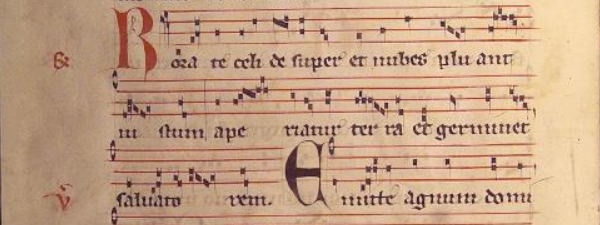
\includegraphics{manuscript}
\caption{Example of a chant in a manuscript. \cite[id~007553]{cantus_db}}
\end{figure}

